\documentclass[12pt]{article}
\usepackage{geometry}                % See geometry.pdf to learn the layout options. There are lots.
\geometry{letterpaper}                   % ... or a4paper or a5paper or ... 
%\geometry{landscape}                % Activate for for rotated page geometry
\usepackage[parfill]{parskip}    % Activate to begin paragraphs with an empty line rather than an indent
\usepackage{daves,fancyhdr,natbib,graphicx,dcolumn,amsmath,lastpage,url}
\usepackage{amsmath,amssymb,epstopdf,longtable}
\usepackage{paralist} 
\DeclareGraphicsRule{.tif}{png}{.png}{`convert #1 `dirname #1`/`basename #1 .tif`.png}
\pagestyle{fancy}
\lhead{CE 3372 -- Water Systems Design}
\rhead{FALL 2020}
\lfoot{ES 7}
\cfoot{}
\rfoot{Page \thepage\ of \pageref{LastPage}}
\renewcommand\headrulewidth{0pt}


\begin{document}
\begin{center}
{\textbf{{ CE 3372 -- Water Systems Design} \\ {Exercise Set 7}}}
\end{center}

\begingroup
\begin{tabular}{p{2in} p{4.5in}}
Purpose: & Apply rational method by-hand; construct a design storm hyetograph\\
~ & ~ \\
ABET General Criteria 3: & (a) \dots apply knowledge of mathematics, science, and engineering  \\
~ & (e)  \dots solve engineering problems  \\
~ & (k) \dots an ability to use the techniques, skills, and modern engineering tools necessary for engineering practice. \\
%~ & ~ \\
%%%Grading Criteria:  & Completion; Correct Solutions; Calculation Details \\
\end{tabular}
\endgroup
\section*{\small{Exercises}}
\begin{enumerate}
%%%%%%%%%%%%%%%%%%
\item A square shaped 250 acre, single family residential area in Harris County ranges in elevation of 150-feet at the North corner to 139-feet at the South corner outlet as depicted on Figure \ref{fig:watershed.jpg}.

\begin{figure}[h!] %  figure placement: here, top, bottom, or page
   \centering
   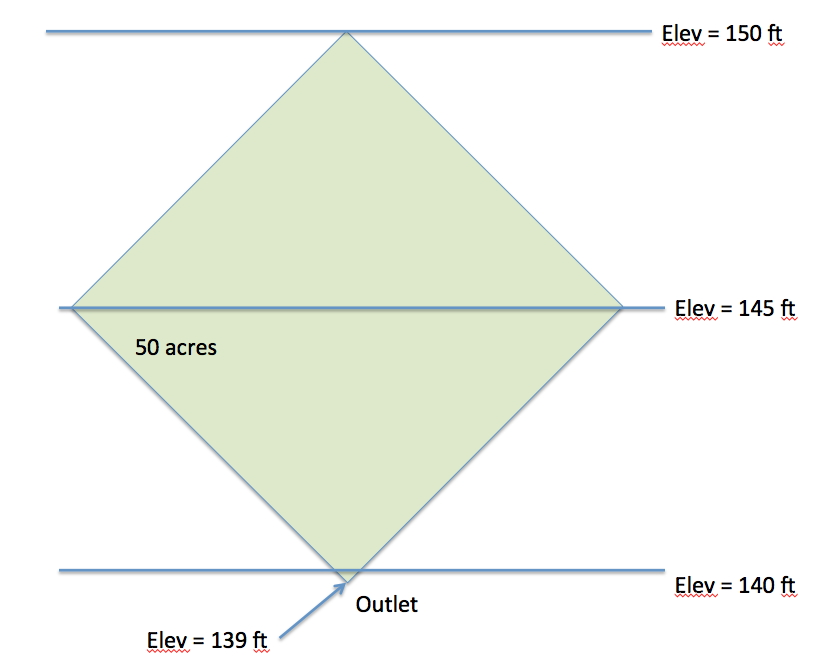
\includegraphics[width=5in]{watershed.png} 
   \caption{250 acre square watershed with land surface elevation points indicated}
   \label{fig:watershed.jpg}
\end{figure} 
\clearpage

\begin{enumerate}[a)]
\item Create an elevation contour map for the study area -- the shaded area is square, 250 acres total area.
\item Draw representative overland flow paths on the map (or diagram)
\item Draw on the diagram the longest flow path from the highest elevation to the outlet that lies within the 250 acre study area.
\item Draw on the diagram the shortest flow path from the highest elevation to the outlet that lies within the 250 acre study area.\item Determine the length, in feet, of both flow paths.
\item Determine the average dimensionless slope along each flow path.
\item Estimate the time of concentration using NRCS upland method.
\item Using the NOAA Atlas 14, Volume 10 for Texas estimate the rainfall intensity for a 10-year ARI, 3-hour duration storm.
\item Using (and citing) a runoff coefficient table, specify the runoff coefficient for the sub-catchment.
\item Estimate the peak discharge for the sub-catchment for a 10-year ARI using the Rational Method.
\end{enumerate}
%\item Using NOAA Atlas 14, Volume 10 for Texas estimate the cumulative rainfall depth for a 10-year, 3-hour storm.
\item Using the SCS Tabulation or TXHYETO, construct from the 10-year, 3-hour storm a design hyetograph at 15 minute intervals.
%\footnote{You will re-use the hyetograph in a subsequent exercise set, so save your work from this exercise on your computer.}



%\item A grass-lined roadside swale (ditch) is to be built as a trapezoidal channel to carry 20 cubic-feet per second, with a 1 foot freeboard.   If the desired flow depth is 1 foot, and the right of way available to fit the ditch is 12 feet, what is the required side slope and bottom width.   The longitudinal slope is 1\%.
%\begin{enumerate}[i]
%\item Sketch the cross section and label the width, depth, and side slope.
%\item Write the appropriate relationships between velocity, depth, and discharge for the section.
%\item Compute the required side-slope in the section.
%\item Compute the mean section velocity in the section.
%\end{enumerate}

\end{enumerate}
\end{document}  